\chapter{Verfahren zur Realisierung von Überdeckungen in Augmented Reality durch Tiefen\-informationen} \label{sec:optimization}


Die folgenden Abschnitte widmen sich den Verfahren zur möglichen Realisierung von Überlagerungen durch Tiefen- und Bildinformationen. Nach der Recherche zu möglichen Verfahren soll erst einmal der Grundlegende Ansatz von \citet{wloka1995resolving} zur einfachen Überlagerung durch Tiefeninformationen mit Hilfe der Projektion der von Project Tango gelieferten Pointcloud realisiert werden, da dieses Ausschlussverfahren das grundlegende Vorgehensmodell zur Überlagerung darstellt. 

Die Kanten und Modell basierenden Verfahren zur AR Überdeckung aus Kapitel \ref{sec:ar-occlusion} werden hier nicht weiter berücksichtigt, da sie offensichtliche Nachteile gegenüber anderen Ansätzen bergen. So muss bei Modell basierten Verfahren bereits ein Modell der echten Umgebung existieren und die Kanten basierte Verfahren schränkt den Einsatz auf eine weniger komplexe Szene ein. Außerdem sind beide Verfahrensarten so konzipiert, dass sie keine direkten Tiefeninformationen benötigen, die aber von Project Tango generiert werden können. Aus diesem Grund widmen sich die darauf folgend beschriebenen Umsetzung der Rekonstuktions basierten Verfahren.

Während dieser Arbeit wurde zunächst versucht ein eigenes Echtzeit Rekonstuktionsverfahren, basierend auf einer Ebenenerkennung zu entwickeln, welches auch auf der beschriebenen mobilen Project Tango Hardware realisierbar ist. Daraufhin wurde nach weiteren Recherchen ein neuer möglicher Rekonstruktionsmechanismus gefunden, der für den Einsatz auf mobiler Hardware konzipiert wurde. Auch dieser wird hier näher beschrieben, um ihn später zu implementieren und zu testen. Zuletzt soll näher auf die Möglichkeit eingegangen werden, die resultierenden Tiefeninformationen aus der Pointcloud oder aus dem Rendering der Rekonstruktion mit Hilfe der Bildaufnahmen der Farbkamera, zu verbessern. 


\section{Verdeckung durch Depth Maps}

\section{Planare Rekonstruktion} \label{sec:plane-reconstruction}

Dieses Kapitel widmet sich der Idee, eine Rekonstruktion für ein  Überlagerungs\-verfahren durch eine Ebenendetektion zu realisieren. \citet{yang2010plane} erwähnen hierzu, dass Ebenen in fast allen künstlichen Umgebungen zu finden sind und aufgrund ihrer vorteilhaften geometrischen Eingenschaften in verschiedensten Computer Vision Verfahren verwendet werden. Daher gibt es viele Forschungsarbeiten, Methoden und Algorithmen, um aus verschiedensten Informationsquellen ein Ebenenmodell zu extrahieren.

Das \enquote{Simultaneous Localization and Mapping} (SLAM) Verfahren von \citet{trevor2012planar} detektiert Ebenen mit dem RANSAC Algorithmus. RANSAC bietet gegenüber anderen Algorithmen zur Ebenendetektion den Vorteil, ein Modell auch bei vielen Ausreißern performant ermitteln zu können. Agglomeratives Clustering und Region Growing wie von \citet{feng2014fast} beschrieben, eignet sich aufgrund des Ausgabeformats von Project Tango nicht direkt, da es keine organisierte Point Cloud ausgibt und die Daten durch Reflektionen und Löcher stärker mit Fehlern behaftet sind. 

Das selbst zusammengestellte Verfahren zur Ebenendetektion besteht daher aus folgenden Komponenten: Wie in dem Ansatz von \citet{yang2010plane} wird der RANSAC Algorithmus auf Würfeln ausgeführt, die eine Menge gesammelter Punkte aus der Pointcloud beinhalten. Dabei entsprechen die Würfel den untersten Knoten eines Octrees, welcher hier zur Speicherung und Aufnahme aller Punkte verwendet wird. Diese untersten Knoten des Octrees werden folgend auch Cluster genannt. Eine gefundene Ebene in einem Würfel wird wie im SLAM Verfahren von \citet{trevor2012planar} persistiert. Die Repräsentation der Ebene \(P\) wird dort wie in Gleichung \ref{eq:plane} festgehalten. Dabei handelt es sich um den Normalenvektor \(\vec{n}\) und der Distanz zum Ursprung \(d\) der Hesse Normalform einer Ebene, sowie der Punkte der konvexen Hülle \(H\). \citet{trevor2012planar} erläutern, dass die konvexe Hülle in der Repräsentation festgehalten wird, um eine sukzessive Verbesserung einer Ebene nach mehreren Messdurchläufen zu ermöglichen. So werden die Punkte der konvexen Hülle pro Messvorgang kombiniert, damit die Ebenenausbreitung auch außerhalb des Sichtfeldes beibehalten werden kann. 

\begin{equation} \label{eq:plane}
P=\left[\vec{n}, d, H\right] \qquad H=\vec{h_1}, \vec{h_2}, \ldots  \vec{h_n}
\end{equation}

Die einzelnen Schritte des Vorgehens werden in den folgenden Absätzen näher erläutert. Ein grober Ablauf des Vorgehens wird aber bereits in Listing \ref{lst:planeReconstruction} zusammengefasst und in Pseudocode beschrieben. 

\begin{lstlisting}[mathescape,caption=Planare Echtzeitrekonstruktion, label=lst:planeReconstruction, float=htbp]

Eingabe: Octree $O$, Anzahl der zu suchenden Ebene in Clustern $N$
Ausgabe: Polygonpunkte $T_{Gesamt}$

für jedes Cluster $C$=[$C_{Punkte}$, $C_{Ebenen}$] aus $O$
    führe $N$ mal aus
        bestimme Ebene [$\vec{n}$, $d$, $P$] mit RANSAC aus $C_{Punkte}$
        wenn keine Ebene mit genügend $P$ gefunden wurde
            nächstes Cluster (continue)
        wenn Ebene mit [$\vec{n}$, $d$, $H_{alt}$] in $C_{Ebenen}$ existiert	
            füge die konvexe Hülle $H_{alt}$ zu $P$ hinzu	
        bestimme die konvexe Hülle $H_{neu}$
        trianguliere $H_{neu}$ zu $T_{Ebene}$
        $T_{Gesamt}$ += $T_{Ebene}$
        $C_{Ebenen}$ += [$\vec{n}$, $d$, $H_{neu}$]
        $C_{Punkte}$ - $P$
\end{lstlisting}


\subsection{RANSAC zur Ebenendetektion} \label{sec:ransac}

Um mit dem RANSAC Algorithmus, beschrieben in Kapitel \ref{sec:ransac-theory}, Ebenen in einer Punktewolke bestimmen zu können, werden pro Iteration drei Stichproben \(\vec{A}\), \(\vec{B}\) und \(\vec{C}\) gewählt, die zur Bestimmung einer Ebene ausreichen. Das Ebenenmodell, hier in der Hesse Normalform mit dem Normalenvektor \(\vec{n}\) und dem Abstand zum Koordinatenursprung \(d\), lässt sich dabei durch die Gleichung \ref{eq:normalform} bestimmen.

\begin{equation}\label{eq:normalform}
\vec{n} =\left|\left| \vec{AB} \times \vec{AC}\right|\right|
\qquad
d = \vec{A} \cdot \vec{n}
\end{equation}

Um zu ermitteln, ob ein weiterer Punkt \(\vec{P}\) aus der Pointcloud eines Clusters die gefundene Ebene \(\left[\vec{n}, d\right]\) unterstützt, wird die kürzeste Distanz \(d_P\) zwischen Punkt und Ebene wie in Gleichung \ref{eq:plane-distance} ermittelt.  Ein entsprechender Toleranzwert für die Distanz \(d_{min}\), im gezeigten RANSAC Algorithmus \(e\) genannt, wird später bei der Umsetzung abhängig von der Ungenauigkeit des Tiefensensors gewählt. 

\begin{equation} \label{eq:plane-distance}
d_P = \vec{n} \cdot \vec{P} - d \qquad support_{d_P} = d_P < d_{min}
\end{equation}

Um das finale Modell der Ebene zu bestimmen, wie im ursprünglichen RANSAC Algorithmus in Punkt 7. aus Listing \ref{lst:planeReconstruction} beschrieben, und somit die Varianz des Abstands der Punkte zur Ebene zu minimieren, wird mithilfe der unterstützenden Punkte \(P_{s}=\left[x,y,z\right]\) eine lineare Regression durchgeführt. Diese mittelt ein Ebenenmodell \(E=\left[\vec{n}, d\right]\) aus den zuvor ermittelten Punkten mithilfe der Methode der kleinsten Quadrate. \citet{hoppe1992surface} nutzen dazu für eine ähnliche Problemstellung die Eigenwert-Dekomposition der Kovarianzmatrix der Punkte \(P_{s}\) zum Zentrum \(\vec{p_{c}}\). In Gleichung \ref{eq:centroid} wird das Zentrum aus den unterstützenden Punkten \(P_{s}\) bestimmt. Gleichung \ref{eq:covarianz} zeigt die Bestimmung der Kovarianzmatrix \(CV\) im Bezug zum Zentroid, in der \(\otimes\) für das dyadische Produkt\footnote{Wenn \(\vec{a}\) und \(\vec{b}\) die Komponenten \(a_i\) und \(b_j\) beinhalten, resultiert aus \(\vec{a} \otimes \vec{b}\) eine Matrix mit den Komponenten \(a_ib_j\) an der \(ij\) Position. \citep{hoppe1992surface}} steht.

\begin{equation} \label{eq:centroid}
\vec{p_{c}} = \frac{\sum_{n=0}^{|P|} \vec{p_{n}}}{|P|}
\end{equation}

\begin{equation} \label{eq:covarianz}
CV = \sum_{n=0}^{|P|} ( \vec{p_{n}}- \vec{p_{c}}) \otimes ( \vec{p_{n}}- \vec{p_{c}})
\end{equation}

Wendet man nun auf der Kovarianzmatrix \(CV\) die Eigenwert-Dekomposition an, erhält man die Normale \(\vec{n}\) aus dem Eigenvektor \(||\vec{v_i}||\) mit dem kleinsten Eigenwert \(\lambda_i\). Somit würde bei \(\lambda_1 \geqq \lambda_2 \geqq \lambda_3\) die Zuweisung \(\vec{n} = ||\vec{v_3}||\) folgen. Die Distanz zum Ursprung \(d\) entspricht dem Kreuzprodukt aus dem Zentroiden \(\vec{p_c}\) und der neu gewonnen Normalen \(\vec{n}\). \citep{hoppe1992surface} 

\subsection{Bestimmung der Ebenenausbreitung}

Nachdem die Ebene und die korrespondierenden Punkte zur Ebene gefunden wurden, muss noch die Ausbreitung der Fläche bestimmt werden, da die Ebene in Hesse Normalform lediglich die Position \(\vec{n} * d\) und Ausrichtung \(\vec{n}\) festhält. \citet{PlanarSurfaceMapping} nutzt hierfür die konvexe Hülle der korrespondierenden Punkte und trianguliert diese. Wie diese Triangulation genau bestimmt wird, wurde von \citet{PlanarSurfaceMapping} nicht beschrieben. 

Um diese Bestimmung performant umsetzen zu können, kann man sich die Eigenschaft der Ebene zunutze machen und die dreidimensionalen Punkte durch Parallelprojektion als zweidimensionale Punkte auf die gefundene Ebene projizieren. Denn die Triangulation ist nach dem Erhalten der zweidimensionalen konvexen Hülle, wie im Listing \ref{lst:triangulation} beschrieben, direkt bestimmbar. Nach der Triangulation können die Ecken der gefundenen Polygone jeweils zurück projiziert werden. Die Gleichungen \ref{eq:projection2d} und \ref{eq:projection3d} bilden die Projektion der Punkte wobei \(R_{\vec{n} \rightarrow \vec{z}}\) der Rotationsmatrix zwischen dem Normalenvektor \(\vec{n}\) und der Z-Achse \(\vec{z}\) entspricht.

\begin{equation} \label{eq:projection2d}
p_{2d} = (p_{3d} - (\vec{n}*d)) * R_{\vec{n} \rightarrow \vec{z}}
\end{equation}
\begin{equation} \label{eq:projection3d}
p_{3d} = (p_{2d} * R_{\vec{n} \rightarrow \vec{z}}^{-1}) + (\vec{n}*d)
\end{equation}

\begin{lstlisting}[mathescape,caption=Bestimmung der Ebenenausbreitung und Triangulation, label=lst:triangulation, float=htb]

Eingabe: Unterstützende Ebenenpunkte aus RANSAC $P$
         Transformation $R_{\vec{n} \rightarrow \vec{z}}$
Ausgabe: Polygone $T_{Ebene}$

    Projiziere alle Punkte aus $P_s$ mit $R_{\vec{n} \rightarrow \vec{z}}$ zu $P_{2d}$
    Bestimme die konvexe Hülle $H$ aus $P_{2d}$ mit Graham Scan
    starte mit leerer Menge $P_{2dmesh}$
    für $i$ von $0$ bis $|H| - 2$
        füge $H_0$ zu $P_{2dmesh}$ hinzu
        füge $H_{i+1}$ zu $P_{2dmesh}$ hinzu
        füge $H_{i+2}$ zu $P_{2dmesh}$ hinzu
    Projiziere alle Punkte aus $P_{2dmesh}$ mit $R_{\vec{n} \rightarrow \vec{z}}^{-1}$ zu $P_{3dmesh}$   
\end{lstlisting}

In Abbildung \ref{fig:polygon-process} ist der Gesamtprozess für die Bestimmung der Ebenenausbreitung veranschaulicht. Nachdem eine Ebene mit RANSAC detektiert wurde, werden die korrespondierenden Punkte auf diese zweidimensionale Ebene projiziert. Daraufhin wird die konvexe Hülle gebildet und die Triangulation der Hülle bestimmt. Diese Polygon Eckpunkte werden danach wieder zurück in den dreidimensionalen Raum projiziert.

\begin{figure}[h]
  \centering
	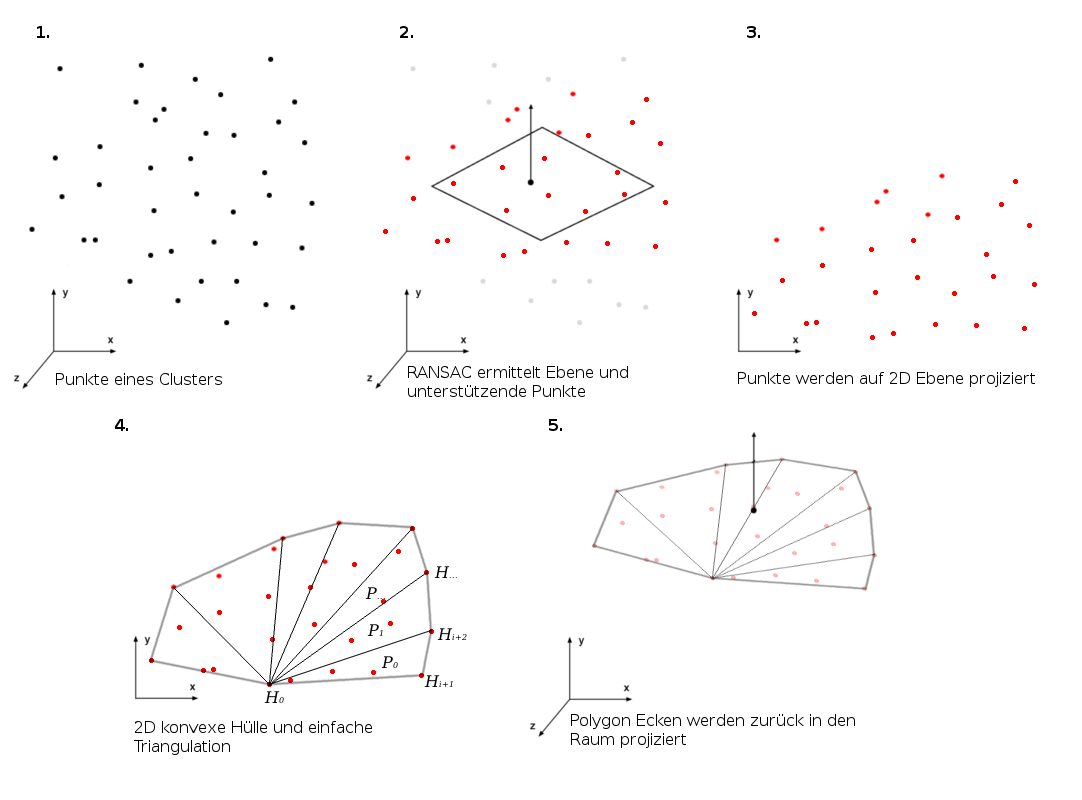
\includegraphics[width=1.1\textwidth]{content/images/methods/polygon-process.png} 
  \caption{Veranschaulichung des Gesamtprozesses zur Bestimmung der Ebenenausbreitung durch RANSAC und der konvexen Hülle.}
  \label{fig:polygon-process}
\end{figure}

\newpage

\subsection{Clustering der aufgenommenen Punkte} \label{sec:cluster}

Wie im Listing \ref{lst:planeReconstruction} zu erkennen, wird das zuvor beschriebene Vorgehen für die planare Rekonstruktion immer pro Cluster eines Cluster-Pools durchgeführt. Dadurch werden pro Durchgang des Algorithmus nur ein Bruchteil der gesammelten Punkte rekonstruiert, was wiederum eine Rekonstruktion in Echtzeit möglich macht. Außerdem verhindert das Clustering das Bilden von konvexen Hüllen über Ebenen, die in Zwischenbereichen nicht mit genügend Punkten unterstützt werden. Dieses Problem ist in Abbildung \ref{fig:clustering} links zu sehen, in welcher eine blaue Ebene rekonstruiert wird, die sich über einen Durchgang ohne vorhandene Punkte streckt.

\begin{figure}[h]
  \centering
	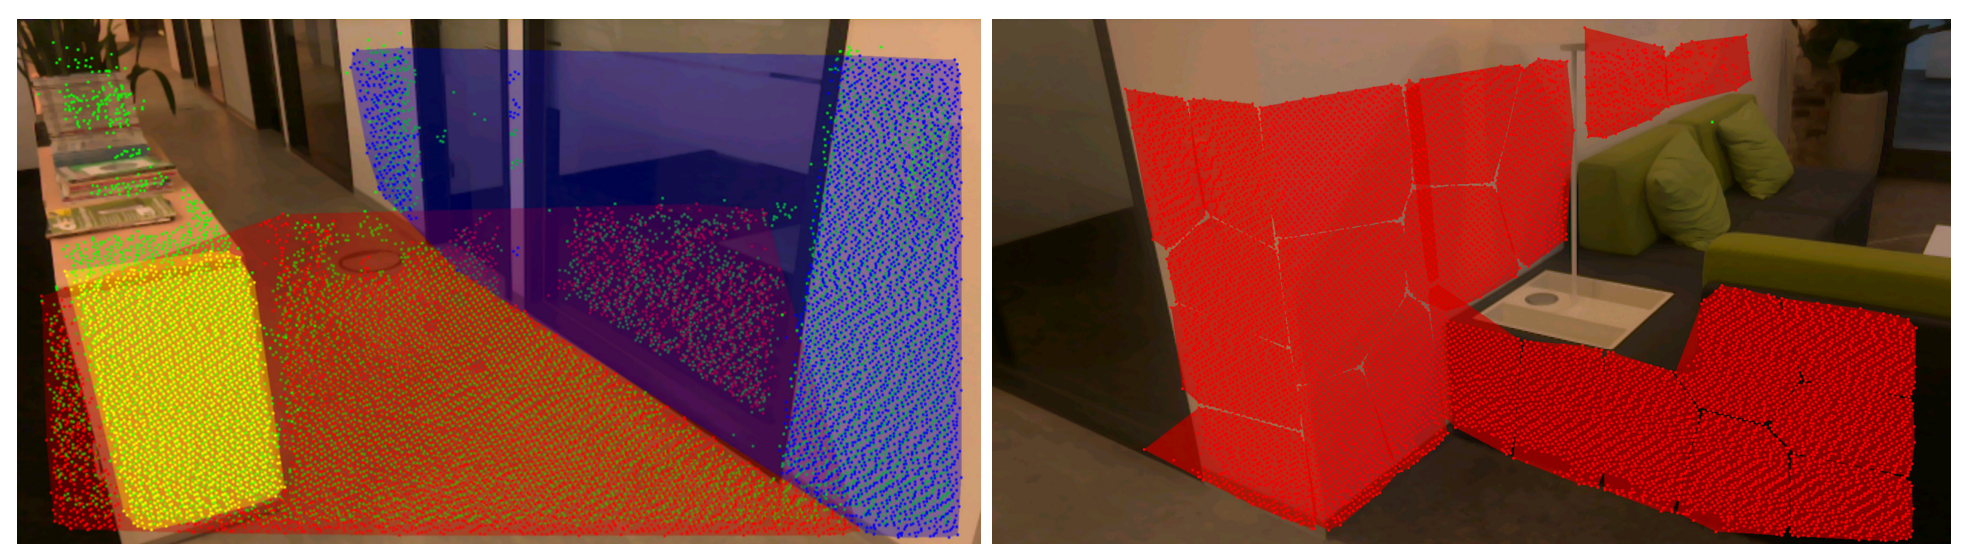
\includegraphics[width=1.0\textwidth]{content/images/methods/clustering.png} 
  \caption{Links: Ebenenrekonstruktion ohne Clustering. Rechts: Rekonstruktion mit K-Mean Clustering.}
  \label{fig:clustering}
\end{figure}

Getestet wurden hier das K-Mean Clustering, Agglomeratives Clustering und einfaches räumliches Clustern mithilfe eines Octrees. Das K-Mean Clustering hat, wie in Abbildung \ref{fig:clustering} rechts zu erkennen, gute Ergebnisse für die Aufteilung einer Ebenen geliefert, benötigt aber zuvor eine feste Anzahl von Clustern. Agglomeratives Clustering, getestet mit dem euklidischen Distanzmaß, würde zwar die Anzahl der Cluster dynamisch bestimmen, ist jedoch zu aufwändig für eine Echtzeitanwendung, wenn dieses auf die gesamten Messergebnisse durchgeführt wird. Ein Einsatz vom K-Mean oder Agglomerativen Clustering ist mangels Skalierbarkeit also nicht möglich.

Gute Ergebnisse liefert wiederum ein einfaches räumliches Clustern mit einem Octree, welcher die aufgenommenen Punkte direkt in Knoten des Baums zuweist. Das bietet zudem den Vorteil, dass diese Datenstruktur direkt als Speicherort der aufgenommenen Punkte und Ebenen dienen kann. Außerdem entspricht dies dem Vorgehen für die Anwendung von RANSAC auf Würfeln, welches von \citet{yang2010plane} beschrieben wurde. 


\section{Polygon Rekonstruktion}

\subsection{Marching Cubes}

\subsection{Possion Reconstruction}

\subsection{Greedy Projection Triangulation}



\section{Tiefenanpassungen durch Farbbilder}

Aus allen zuvor beschriebenen Verfahren werden letztendlich Tiefeninformationen, in Form von geometrischen Primitiven oder Punkten im Raum gewonnen. Diese werden passend zur aktuellen Kameraposition als Tiefenbild gerendert und füllen den Z-Buffer für eine entsprechende Aussparungen bei der Überdeckung virtueller Objekte. Auf Grund von Sensorungenauigkeiten und größeren Auflösungen der Rekonstruktionsverfahren können dabei fehlerhafte Tiefeninformationen im Z-Buffer gelangen, die zu Fehlern bei der Bestimmung der Überdeckung führen können. Dieses Problem ist am Beispiel der Pointcloud Projektion aus Kapitel \ref{sec:pc-projection} in Abbildung \ref{fig:pc-noise} zu erkennen. 

\begin{figure}[h]
  \centering
	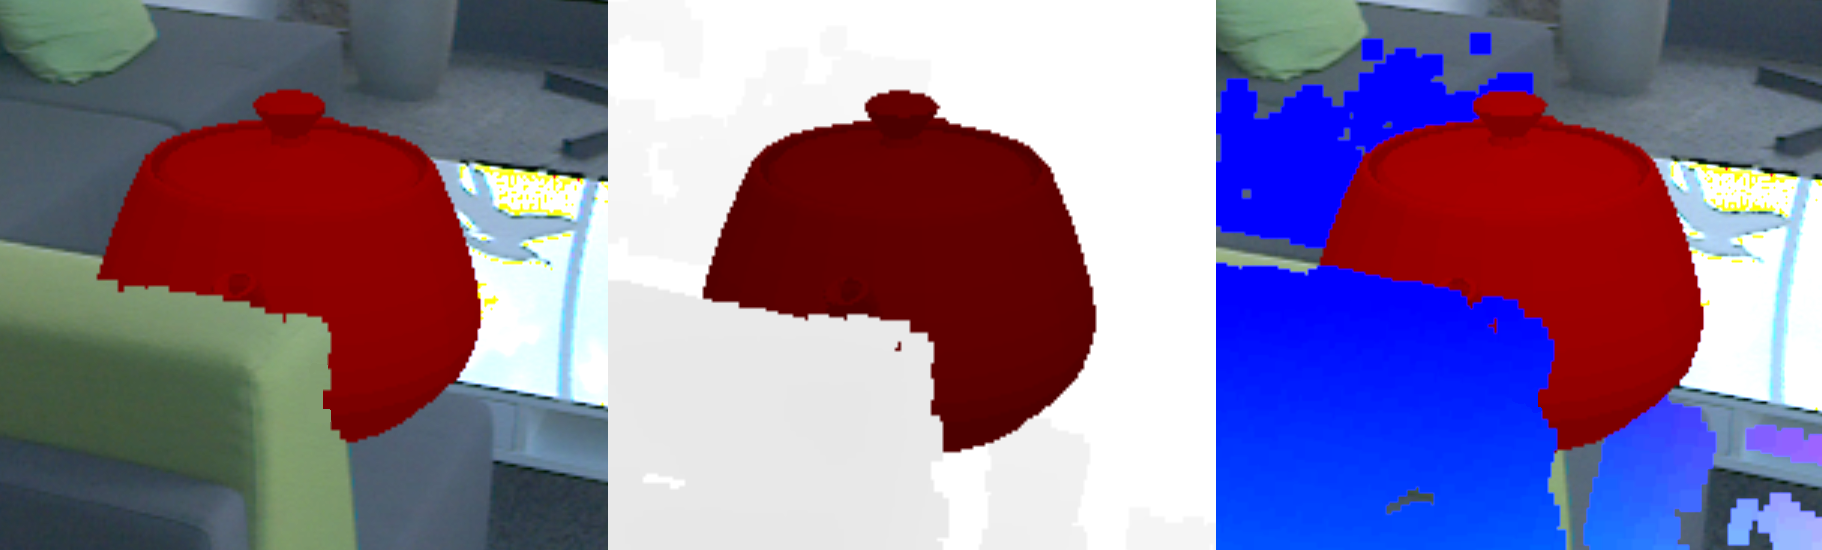
\includegraphics[width=1.0\textwidth]{content/images/methods/pc-noise.png} 
  \caption{Überdeckung mit einfacher Pointcloud Projektion. Links: Resultat der Überdeckung. Mitte: Darstellung des Tiefepuffers. Rechts: Darstellung der Pointcloud.}
  \label{fig:pc-noise}
\end{figure}

Die Reduktion von Ungenauigkeiten im Tiefenbild könnte durch einen einfachen Weichzeichner erreicht werden. Dieser würde jedoch die Kanten im Farbbild nicht berücksichtigen und somit fehlerhafte Tiefengradienten an den Kanten erzeugen und einen durchaus größeren Fehler generieren. \citet{newcombe2011kinectfusion} wenden einen sogenannten \enquote{Bilateralen Filter} in ihrem KinectFusion Rekonstruktionsverfahren an, bevor sie die Tiefeninformationen in die TSDF Repräsentation einfließen lassen. Dieser Filter von \citet{tomasi1998bilateral} ermöglicht das Weichzeichnen ohne dabei die Kanten im Bild zu übergehen, bezieht sich jedoch nur auf das selbe Bild, auf dem der Filter angewendet wird. 

\citet{liu2012guided} hingegen wenden einen sogenannten \enquote{Guided Filter} in Ihrem Verfahren zur Optimierung der der Tiefeninformationen für Kinect ähnliche Sensoren auf das Tiefenbild an. Dieser Filter von \citet{he2010guided} ist in der Lage, auf Grundlage eines anderen Leitbildes ein Weichzeichnen durchzuführen, ohne dabei die Kanten des Leitbildes zu überschreiten. Auch wenn \citet{petschnigg2004digital} eine Erweiterung, den Joint Bilateral Filter, vorstellen, der auf Basis eines anderen Leitbildes eine Weichzeichnung ohne Kantenüberschreitung ermöglicht, bietet der Guided Filter eine deutlich bessere Performance. Außerdem verhindert der Guided Filter Fehlerartefakte im Resultat, die bei dem Bilateralen Filter an den Kanten auftreten können. \citep{he2010guided} 

Ausgehend von der Eingangsgrafik \(p\), einem Leitbild \(I\) und dem Ergebnisbild \(q\) wird das grundlegende Modell dieser Art von Filter mit der Gleichung \ref{eq:gf-model} beschrieben. Diese Gleichung findet für jeden Pixel \(i\) in \(q\) eine gewichtete Summe über jeden Pixel \(j\) einer vordefinierten Ausschnittgröße. \(W_{ij}\) entspricht dabei dem Gewicht, welches für die jeweiligen Pixel \(p_j\) gilt. Bei dieser Faltung gilt üblicherweise  \(\sum_{j} W_{ij}(I)=1 \forall i \in [1\ldots |p|]\). \citep{he2010guided}

\begin{equation} \label{eq:gf-model}
q_{i} = \sum_j W_{ij}(I)p_j
\end{equation}

Der Filterkern \(W_{ij}(I)\) vom Guided Filter, zu finden in Gleichung \ref{eq:gf-W}, ist, wie auch beim bilateralen Filter, abhängig von einem Leitbild \(I\), um die Gewichte entsprechend den Kanten des Leitbildes an der Position ermitteln zu können. Die Variablen \(\mu_k\) und \(\sigma^2_k\) beschreiben jeweils den Mittelwert und die Abweichung des Leitbildes im Bildausschnitt \(w_k\). \(|w|\) entspricht der Pixelgröße des Ausschnitts. \citep{he2010guided}

\begin{equation} \label{eq:gf-W}
W_{ij}(I) = \frac{1}{|w|^2} \sum_{k:(i,j) \in w_k} (1+\frac{(I_i-\mu_k)(I_j-\mu_k)}{\sigma^2_k + \epsilon})
\end{equation}

Dieser Filterprozess wird auch als eine translationsabhänige Faltung bezeichnet, die üblicherweise aufwändig ist und dessen Berechnungsaufwand abhängig zur Filterkern Größe (\(|w|\)) ist. \citet{he2010guided} stellen jedoch noch eine andere Definition des Filters zur Verfügung, in denen alle Summen der Form \(\sum_i\in w_k f_i\) entsprechen und dadurch mit der Bildintegrationstechnik von \citet{crow1984summed} in \(O(N)\) gelöst werden können. Der Guided Filter wird in der letztendlichen Implementierung nach Gleichung \ref{eq:gf-final} implementiert, in der die Koeffizienten \(\overline{a}_i\) und \(\overline{b}_i\) dem Mittelwert über \(a_k\) aus Gleichung \ref{eq:gf-a} und \(b_k\) aus Gleichung \ref{eq:gf-b} für jedes Fenster \(w_k\) entspricht. So wird auch \(\overline{p}_k\) durch \(\frac{1}{|w|} \sum_{i \in w_k} p_i\) berechnet.

\begin{equation} \label{eq:gf-final}
q_i = \overline{a}_iI_i+\overline{b_i}
\end{equation}

\begin{equation} \label{eq:gf-a}
a_k = \frac{\frac{1}{w} \sum_{i \in w_k} I_i p_I - \mu_k \overline{p}_k}{\sigma_k^2+\epsilon}
\end{equation}

\begin{equation} \label{eq:gf-b}
b_k = \overline{p}_k - a_k\mu_k
\end{equation}

Der Faktor \(\epsilon\) reguliert im beschriebenen Filter von \citet{he2010guided} welcher Bildanteil als beizubehaltende Kante im resultierenden Bild gewertet werden soll und somit stärker oder schwächer in die Gewichtung \(W_{ij}\) Einfluss nimmt. Neben diesem Regulierungsfaktor ist auch die Wahl des Radius \(r\) für den Ausschnitt \(w_k\) als Eingabe für diesen Filter wichtig. Der Radius wirkt sich laut \citet{he2010guided} jedoch nicht wie beim bilateralen Filter auf die Laufzeit des Filters aus. 

\begin{quote}
\enquote{One more advantage of the guided filter over the bilateral filter is that it automatically has an \(O(N)\) time exact algorithm. \(O(N)\) time implies that the time complexity is independent of the window radius \(r\), so we are free to use arbitrary kernel sizes in the applications.} \citep{he2010guided}
\end{quote}

\begin{figure}[h]
  \centering
	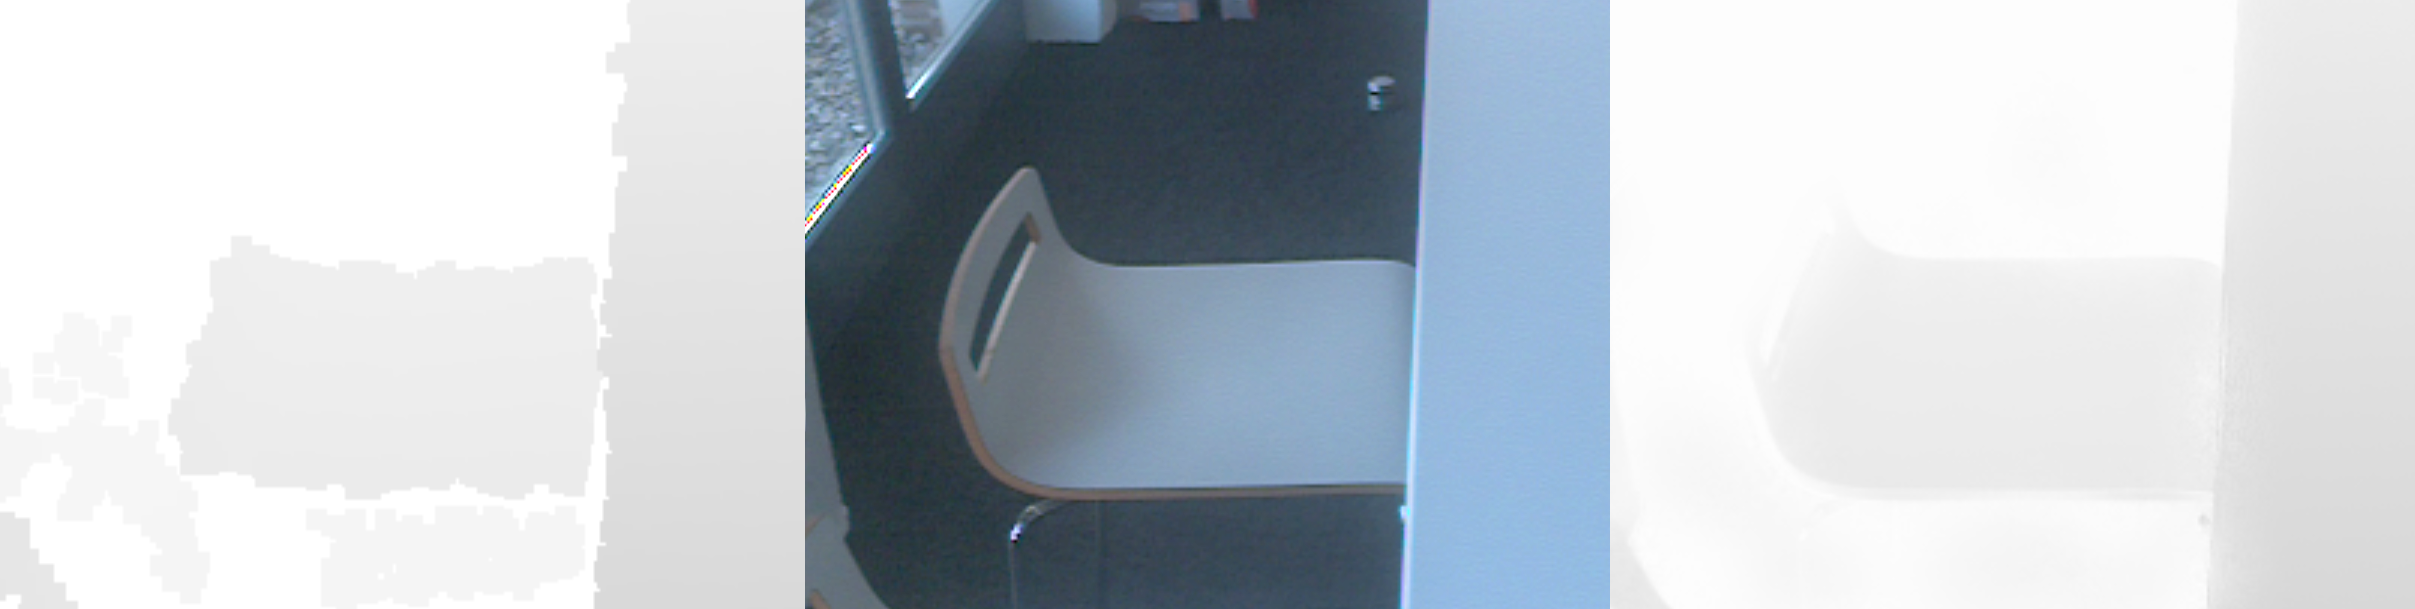
\includegraphics[width=1.0\textwidth]{content/images/methods/gf-result.png} 
  \caption{Guided Filter Anwendungsbeispiel. Das Tiefenbild links ergibt durch den Guided Filter mit dem Leitbild in der Mitte das Ergebnis im rechten Bild.}
  \label{fig:gf-result}
\end{figure}

Mit einer Komplexität von \(O(N)\) findet dieser Filter erfolgreich Anwendung in verschiedensten Bereichen. Er wird zum Beispiel zur Rauschunterdrückung, dem Weichzeichnen oder Verstärken von Details, zur HDR Kompression, dem Entfernen von matten Bildeigenschaften oder, wie in diesem Fall, zum zusammengeführten Anreichern von Bildinformationen verwendet \citep{he2010guided}. Angewendet auf das ermittelte Tiefenbild kann dieser Guided Filter, mit dem jeweiligen RGB Bild als Leitbild, ein Rauschen eliminieren und die Kanten der Tiefeninformationen durch ein entsprechend groß gewählten Fensterradius \(r\) und Regulierungsfaktors \(\epsilon\), an die Kanten der Kameraaufnahme angleichen \citep{liu2012guided}. Ein Beispiel für eine erfolgreiche Anwendung dieses Filters ist in Abbildung \ref{fig:gf-result} zu sehen.



